\chapter{Las bases de la electricidad}
\section{¿Qué es la electricidad?}
Con un poco de teoría, voy a explicar algunos conceptos básicos
para que entiendas lo que es la electricidad.
Así podrás medir y probar muchos de los componentes de tus
en tus electrodomésticos.

\begin{figure}[h]
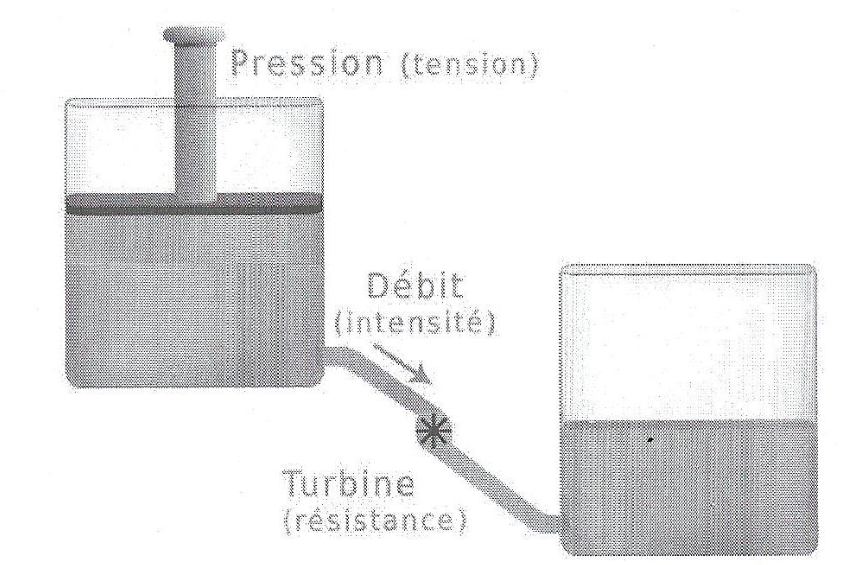
\includegraphics[width=0.8\textwidth]{analogia-agua-elec} 
\caption*{Analogía entre la electricidad y el agua}
\end{figure}

\begin{itemize}
\item \textbf{La tensión (U)} se expresa en voltios (V). Puede ser \textbf{Contínua}, como en una batería, salida del cargador, etc.) o \textbf{Alterna} (señales de la red eléctrica
señales electrónicas, etc.). Es una diferencia de potencial eléctrico entre dos
dos puntos. Siempre medimos una tensión entre dos puntos. Veremos más tarde cómo hacerlo. La tensión de una batería puede ser de 1.5V, 3V, 9V, la tensión de red ronda actualmente los 230V.

\item \textbf{La intensidad (I)} (o "corriente") se expresa en amperios (A).
Flujo de electrones a través de un hilo conductor con una determinada impresión.
A diferencia de la tensión, para que exista una corriente debe consumirse energía.
debe consumirse energía. ë
No hay corriente medible en una pila que no está conectada a nada.
- En este caso, decimos que no tiene "carga" (lo que no significa que no esté cargada en el sentido de que no esté conectada a nada).
 que no esté cargada en el sentido de una pila descargada, significa que
que no está suministrando energía).

\item \textbf{La resistencia (R)} se expresa en ohmios $\Omega$. Es muy baja
(a menudo se considera nula) para los metales y muy alta para el aire
el aire, el plástico o la madera seca, por ejemplo.
Por tanto, un cable eléctrico tendrá una resistencia muy cercana a 0$\Omega$ y el aire tendrá
una resistencia considerada infinita.
Algunos componentes electrónicos o elementos eléctricos también se denominan "resistencias"
o elementos eléctricos (por ejemplo, la resistencia de un horno eléctrico
horno o tostadora).
También existen resistencias "variables", ya sea por acción mecánica o por un cambio de temperatura.
o por un cambio de temperatura, por ejemplo.

\end{itemize}

\noindent\fbox{%
    \parbox{\textwidth}{%
La relación entre estos tres valores es $U(V) = R(\Omega) \times I(A)$, lo que implica que para una tensión fija, si disminuye la resistencia, la intensidad aumenta, y vice versa. Esto se comprende bien gracias al esquema de analogía entre el agua y la electricidad!
    }%
}\\

Para medir estos tres valores eléctricos, necesitamos una herramienta especial llamada "multímetro". (véase el capítulo 2.4).

\begin{figure}[h]
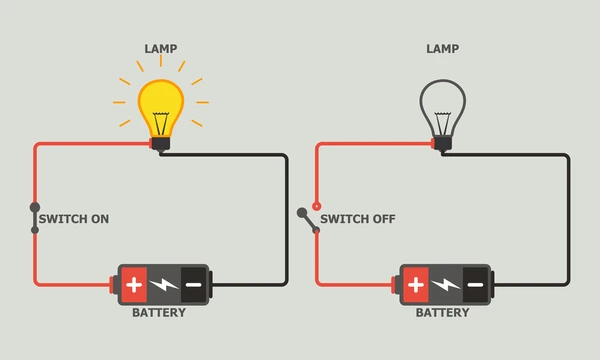
\includegraphics[width=0.7\textwidth]{circuito-abierto-cerrado} 
\centering
\caption*{Circuito abierto o cerrado (cambiar por otra figura)}
\end{figure}

\begin{enumerate}
\item Interruptor cerrado: la tensión "U" es igual a la tensión del generador, y ésta se extiende hasta los contactos de la lámpara (la tension en los extemos de un cable o de un interruptor cerrado siempre es de 0V). La corriente (I) existe y proporciona corriente a la lámpara para encenderse.
\item Interruptor abierto: la tensión "U" es igual a la tensión del generador, La tensión en los contactos de la lámpara es de 0V, no circula corriente
\end{enumerate}
La analogía con el agua no funciona aquí: un circuito cerrado significa que la electricidad puede circular.
posible circulación de electricidad, mientras que un grifo cerrado significa que no hay
circulación de agua...

\section{Los dispositivos de seguridad eléctrica}

\begin{large}
\textbf{a) Hilos y colores}\\
\end{large}
En primer lugar, para orientarse más fácilmente, hay que saber a qué corresponden los
corresponden en electricidad,
Pero como estos colores no siempre se respetan, veremos más adelante cómo estar seguros.
\begin{enumerate}
\item Para una tensión contínua:
\begin{itemize}
\item El hilo negro será el \textbf{-} (O a menudo el conector exterior en cables blindados)
\item El hilo rojo será el \textbf{+} (O a menudo el hilo conductor interior en cables blindados)
\end{itemize}


\begin{normalize}
Un cable "blindado" es un cable que está envuelto en un blindaje metálico conectado a la masa del aparato, para evitar interferencias electromagnéticas.
\end{normalize}

\item En lo que incumbe a instalaciones eléctricas: no se deje engañar por la posición del neutro y lugar del neutro y la fase en una toma eléctrica, esta norma no siempre se
esta norma no siempre se respeta, ya que si invierte el neutro y la fase, también
también funcionará.

\begin{figure}[h]
    \centering
    \begin{minipage}[b]{0.45\textwidth}
        \centering
        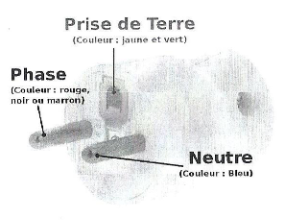
\includegraphics[width=\textwidth]{enchufe-macho} 
    \end{minipage}
    \hfill
    \begin{minipage}[b]{0.45\textwidth}
        \centering
        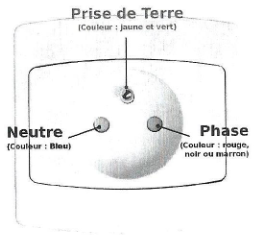
\includegraphics[width=\textwidth]{enchufe-hembra} 
    \end{minipage}
\end{figure}

\begin{itemize}
\item La fase (llegada de la corriente): todos los colores excepto azul y verde/amarillo. Puede estar directamente conectada al tablero de fusibles, o conecetada a un interruptor, por ejemplo
\item El neutro (escape de la corriente): azul
\item La tierra: verde y amarillo
\end{itemize}

\end{enumerate}

\newpage
\textbf{b) ¿De qué sirve la tierra y el disyunctor diferencial?}\\
Es importante comprender la finalidad de estos dos elementos, que han sido
creados para reducir el riesgo de electrocución de las personas en caso de avería de un aparato, como una fuga de agua en una lavadora, por ejemplo (el agua es un buen conductor de la electricidad)

\begin{figure}[h]
\includegraphics[width=0.7\textwidth]{diferencial-protección-tierra} 
\centering
\caption*{\textit{Los diferentes grados de protección de una instalación eléctrica}}
\end{figure}

Imagine un contacto eléctrico entre un cable conectado a un potencial eléctrico peligroso
(como la red de 230 V) y la carcasa metálica de su frigorífico.
de su frigorífico.

\begin{itemize}
\item Caso de la primera imagen: sin tierra ni disyunctor diferencial.
Si un apersona toca el frigorífico, la corriente pasará por el cuerpo de ésta para retornar a la tierra (ya que la corriente de la red está referenciada a tierra y siempre busca volver a ella, un poco como si se sintiese atraída por ella).

\textbf{$\Rightarrow$ La persona se electrocuta}

\item Caso de la segunda imagen: el cable de tierra está presente, es decir
todas las partes metálicas de los aparatos eléctricos están conectadas eléctricamente a tierra, pero sigue sin haber interruptor diferencial.
Esta vez, si alguien toca el frigorífico, la corriente fluirá a través del cable de tierra Y a través del cuerpo de la persona.

\textbf{$\Rightarrow$ La persona se da un calambre}
\newpage

\begin{normalize}
La corriente será mucho menor en el cuerpo de la persona que en el cable de tierra, porque la resistencia eléctrica entre la mano y los pies de una persona es mucho mayor que la de un cable de cobre. Cuanto menor sea esta resistencia (dedos y pies mojados, sobre un suelo húmedo, etc.), mayor será la fuga a tierra. Más fuerte y, por tanto, más peligrosa será la corriente.
\end{normalize}

\item Último caso: incluso antes de que alguien toque el aparato averiado, el disyuntor diferencial detectará la fuga de corriente y cortará la corriente a toda la instalación eléctrica. Se trata de la famosa palanca o botón grande que suele colocarse junto al contador de la luz.

\end{itemize}

\begin{figure}[h]
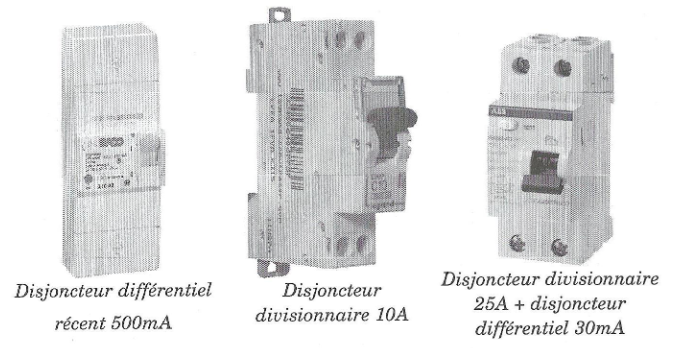
\includegraphics[width=0.9\textwidth]{disyunctores} 
\centering
\end{figure}

El interruptor diferencial mide la corriente que entra en la vivienda a través de la fase y la corriente que sale de la vivienda a través del conductor neutro.
Si la diferencia supera los 500 mA (650 mA en los modelos más antiguos), se dispara.
En ese caso, suele significar que un aparato conectado (no necesariamente en funcionamiento) está averiado.
Los interruptores diferenciales no deben confundirse con los interruptores divisionales.
disyuntores, que ahora sustituyen a los antiguos fusibles.\\

La función de un disyuntor divisor es cortar la electricidad a una parte de la instalación cuando se produce una sobreintensidad en dicha parte, es decir, cuando se produce un sobreconsumo anormal de corriente.
Generalmente, se disparan a los 16A para los enchufes convencionales, a los 10A
para el alumbrado (también los hay de 20A o 32A para alimentar determinados aparatos de alto consumo: cocina eléctrica, termo...).

La causa de esta sobreintensidad puede ser un aparato defectuoso, pero también puede ser el consumo normal de varios aparatos conectados al mismo circuito.
ser el consumo normal de varios aparatos conectados al mismo circuito de
circuito (no necesariamente el mismo enchufe).

\noindent\fbox{%
    \parbox{\textwidth}{%
Ejemplo: un termo eléctrico con una potencia P de 2300W, consumirá una corriente de 10A ($P = U \times I \rightarrow I = P/U = 2300W / 230V = 10A$)
Si enchufais uno o más aparatos sobre el mismo circuito, cuyo consumo sobrepase 6A, el disyunctor divisionario o el fusible de 16A cortará el circuito: $10+6=16A$
    }%
}\\

En las instalaciones recientes, se montan en el mismo módulo un disyuntor y un interruptor diferencial para cada parte de la instalación. Estos disyuntores diferenciales suelen dispararse a 30mA y por una buena razón:

\begin{figure}[h]
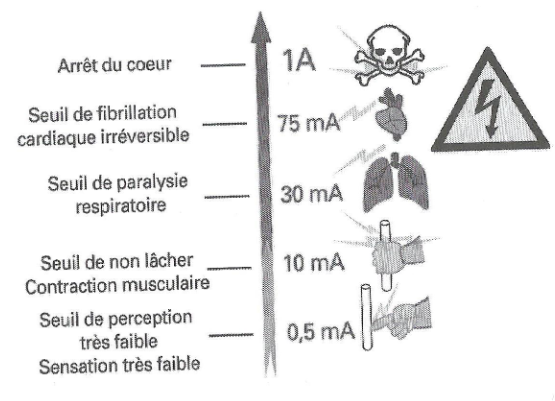
\includegraphics[width=0.9\textwidth]{corriente-efectos} 
\centering
\end{figure}

\textbf{b) ¿Cómo verificar una buena conexión a tierra?}\\
El disyunctor diferencial, está presente hoy en día en la mayor parte de instalaciones eléctricas de España, mientras que la toma de tierra está desgraciadamente ausente en muchas (la presencia de contactos de tierra en el enchufe no implica que esté conectada) Hay que coger el hábito de verificar si la tierra está bien conectada a los enchufes que vamos a usar para nuestros aparatos (sobre todo si hay facilidad de contacto con partes metálicas) Para ello, utilizaremos el multímetro (ver capítulo 2.4) en modo voltímetro en un rango de alterna superior a 240V.
\begin{itemize}
\item Entre el neutro y la fase deberíamos obtener 230V
\item Entre la fase y la tierra igualmente 230V (si no: tierra mal conectada)
\item Entre el neutro y la tierra, no más de 5V (si no: tierra mal conectada)
\end{itemize}
\newpage

Estas mediciones también permiten determinar la ubicación de la fase y el neutro, que no siempre están colocados como se muestra en el diagrama siguiente:

\begin{figure}[h]
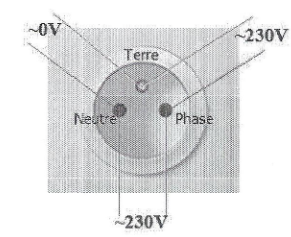
\includegraphics[width=0.4\textwidth]{diagrama-enchufe} 
\centering
\end{figure}

\section{Los peligros eléctricos que podeis encontrar durante las reparaciones}
Si no sabes lo que haces, la electricidad puede ser peligrosa e incluso mortal.
Al solucionar problemas, intentamos evitar trabajar bajo tensión en la medida de lo posible, pero el peligro no siempre se elimina. Me refiero a la tensión de red, los 230V AC. Sin embargo, un dispositivo alimentado por una batería también puede ser peligroso.\\

\textbf{a) Aparato bajo tensión}\\

Como norma general, conecte un aparato a la red sólo para una prueba o medición rápida y desconéctelo inmediatamente después.

\begin{itemize}
\item En caso de medir con el aparato bajo tensión, hay que poner especial atención a no poner los dedos, o cualquier parte del cuerpo en contacto con el aparato, las manos deben de estar sobre las dos puntas del multímetro y lo más alejadas posible de la parte bajo tensión.
\item No se debe tener ningún recipiente con agua u otro líquido a proximidad del aparato y la mesa de trabajo debe estar despejada y limpia.
\item Intentad estar lo más aislado posible del suelo, con buenos zapatos de goma e idealmente una tabla de madera debajo.
\end{itemize}
\newpage

\textbf{b) Aparato sin tensión o alimentado por una pila/batería}\\
Aunque el aparato esté desenchufado, debe tener especial cuidado con
un componente electrónico fácilmente reconocible: el condensador.
\begin{figure}[h]
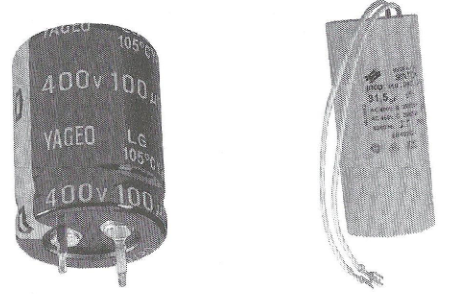
\includegraphics[width=0.7\textwidth]{condensadores} 
\centering
\end{figure}

Estos pequeños cilindros son capaces de almacenar alta tensión, lo que puede ser
peligroso.
Encontrará el modelo de la izquierda soldado a las tarjetas de alimentación de la mayoría de los aparatos más recientes conectados a la red que necesitan tensiones continuas. Pero también lo encontrarás en las cámaras digitales para dar al flash la potencia que necesita. El condensador de la derecha se encuentra en electrodomésticos como las lavadoras. También encontrará un condensador capaz de almacenar una tensión de unos 4000V en los hornos microondas: ¡una alta tensión muy peligrosa!
En ambos casos, la única forma de saber si debe desconfiar es
comprobar la tensión máxima admisible impresa en el componente.
Si supera los 50 V, deberá tomar las precauciones indicadas en el apartado
sección sobre condensadores (véase el capítulo 5.4.2).\\

En resumen, recuerde que los dispositivos potencialmente peligrosos, aunque estén apagados, son :
\begin{itemize}
\item Todos los aparatos alimentados por la red eléctrica equipados con una fuente de alimentación conmutada (véase el cap. 5.3.a)
\item Cámaras digitales
\item Hornos microondas
\item Tubos de rayos catódicos de pantallas y televisores antiguos
\end{itemize}
\newpage

\section{Utilización de un multímetro}
El multímetro es una herramienta electrónica esencial para medir
determinados valores eléctricos. La mayoría de los multímetros actúan como
voltímetro, amperímetro y óhmetro, es decir, miden tensiones
y resistencias, lo que suele bastar para la localización de averías.
resolución de problemas. La mayoría de las veces, lo único que necesitamos es medir tensiones y resistencias. Los multímetros se pueden adquirir por unos diez euros o más y son suficientes para la localización de averías.

\begin{figure}[h]
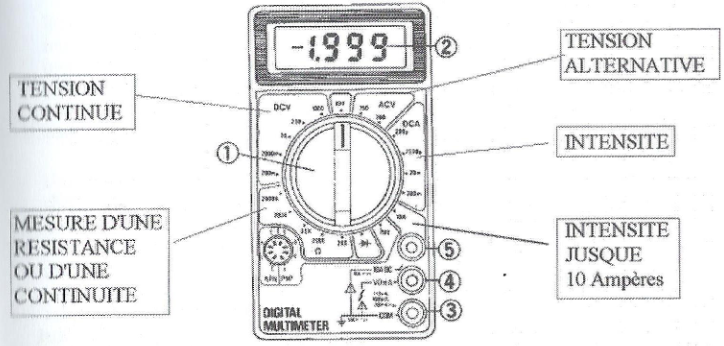
\includegraphics[width=\textwidth]{multimetro-digital} 
\centering
\caption*{\textit{Multímetro digital básico}}
\end{figure}
\textbf{a) ¿Cómo se utiliza?}\\

En primer lugar, con su multímetro, tendrá dos cables, uno rojo y uno negro. En un lado de estos cables, habrá una clavija "banana" que se conecta al multímetro, y en el otro lado, un "punto de contacto" para realizar las mediciones.
El negro se conecta siempre a la clavija "COM" (marcada con un 3 en la imagen) de su multímetro, el rojo puede enchufarse en diferentes puntos dependiendo de lo que quieras medir.
Ten en cuenta que por debajo de unos 50V (en un ambiente seco), no estás arriesgando mucho.
Puedes poner los dedos en los dos polos de una batería tanto como quieras. Sin embargo, ten mucho cuidado cuando estés midiendo tensiones más altas, como la de la red eléctrica, por ejemplo.

\newpage

\textbf{b) Medida de continuidad, de aislamiento y de resistencia}\\

Es muy importante saber medir la continuidad, de hecho es lo más importante
para encontrar la mayoría de los problemas en los equipos eléctricos.
equipos eléctricos.

Gracias a esta medida, podemos comprobar que la mayoría de los elementos eléctricos y ciertos componentes electrónicos.\\

Lo que llamamos "medir la continuidad" es comprobar que existe contacto eléctrico entre dos puntos.
La continuidad equivale a una resistencia prácticamente nula ($\approx$0$\Omega$).

En particular, se utiliza para comprobar que un cable no se ha cortado dentro de su aislamiento, lo que ocurre más a menudo de lo que se cree.
aislamiento, lo que ocurre más a menudo de lo que se piensa.

A la inversa, lo que llamamos "medir el aislamiento" es comprobar que
que no hay contacto entre dos puntos, es decir, que hay una resistencia "infinita".\\

\textbf{
Para medir la continuidad eléctrica o la resistencia, el aparato debe
estar siempre apagado}\\

El multímetro envía una corriente baja para realizar la medición.
Por lo tanto, esta medición es segura. Para comprobar la continuidad entre dos puntos, coloque el multímetro en el valor $\Omega$ más bajo o {\Large \loudspeaker}  si su multímetro dispone de la función "pitar para continuidad" (que le permite comprobar varias continuidades sin tener que mirar la pantalla cada vez).
Coloque sus dos puntas en los dos extremos a comprobar: si la continuidad es
Si la continuidad es buena, obtendrá un valor próximo a 00 y/o emitirá un pitido. Si no hay continuidad (resistencia demasiado alta), no cambiará nada en la pantalla. Mostrará OL (sobre límite) o "1" según el aparato.
Para comprobar la diferencia en pantalla entre continuidad y no continuidad, simplemente junte las dos puntas de su multímetro.Tenga en cuenta los diferentes prefijos: miliohm, ohm, Kohm, Mohm.\\

A veces será necesario comprobar una resistencia infinita.
(Por ejemplo, entre las clavijas que alimentan un elemento eléctrico y su carcasa metálica, debe haber una resistencia infinita).
Debe hacer lo mismo que para medir la continuidad, excepto que debe ajustar el multímetro al valor $\Omega$ más alto. No ajuste el multímetro a la función "continuidad" para esta medición.
El aislamiento se produce cuando no ocurre nada en la pantalla durante la medición.
\newpage

Para medir una resistencia eléctrica, sitúese sobre $\Omega$ y coloque las puntas en las extremidades de la resistencia, si obtiene una resistencia infinita, está cortada y necesita ser reemplazada.
Si obtiene 0 $\Omega$, puede estar en cortocircuito, así que desuelde/desenchufe la resistencia del resto del resto del aparato y mida de nuevo sus terminales para comprobar que está en cortocircuito. Si no es así, el problema está en otra parte del aparato: otra resistencia conectada en paralelo, por ejemplo.\\

\textbf{
c) Medida de la tensión}\\
Aparte de las señales electrónicas más complejas (cuadrada, triangular, modulada....), en las que no entraré en esta guía, hay dos formas de tensión que debes conocer: la tensión continua y la tensión alterna "sinusoidal" de la red eléctrica doméstica.

\begin{itemize}
\item \textbf{La tensión contínua}

\begin{normalize}
Una tensión continua es una tensión estable en el tiempo y que tiene una forma lineal
una pila de 9V (si no tenemos en cuenta que se descarga gradualmente) siempre entregará 9V. 
Para medir una tensión de este tipo, pon tu multímetro en tensión continua
(CC o V=). Si hay varios calibradores (algunos multímetros tienen calibración automática
calibración automática) y no sabe lo que va a obtener, elija el mayor; si obtiene algo como 0,001V, reduzca el calibre hasta que obtenga un valor bastante exacto.
A continuación, simplemente coloque cada una de las puntas de su multímetro sobre los dos contactos a medir, el + y el - de una pila, por ejemplo.
Si las patillas de su multímetro están invertidas, mostrará un "-" delante del
del valor.
\end{normalize}

\newpage


\item \textbf{La tensión alterna sinusoidal}
En contra a una tensión contínua, la tensión alterna tiene una evolución cíclica respecto al tiempo.

\begin{figure}[h]
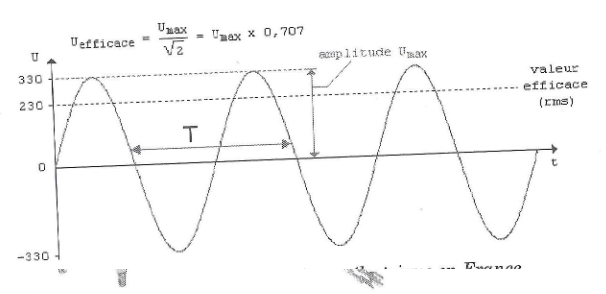
\includegraphics[width=\textwidth]{tension-alterna-sinusoidal} 
\centering
\caption*{\textit{Forma de la tensión de la red eléctrica europea}}
\end{figure}
Tomemos el ejemplo de nuestra red eléctrica, es una tensión sinusoidal de 230V, así que coloque su multímetro en "tensión alterna" (AC o V$\approx$), sobre el primer valor más alto que 230V
A continuación, basta con colocar cada una de las puntas del multímetro en uno de los dos contactos a medir, un enchufe por ejemplo. Si inviertes el + y el - en tu multímetro, no habrá ninguna diferencia. No hay "dirección" en una corriente alterna ya que cambia de dirección regularmente, lo que medimos es lo que llamamos su "valor eficaz".

\noindent\fbox{%
    \parbox{\textwidth}{%
Definición: El valor eficaz de la tensión (llamada "rms"), es el valor de una tensión contínua que tendría los mismos efectos sobre una resistencia eléctrica.
    }%
}\\


\noindent\fbox{%
    \parbox{\textwidth}{%
Esta señal se llama "alterna", porque cambia de signo/sentido, tiene un período (T) que determina la duración del patrón elemental que se reproduce al infinito. Este período (T) se mide en segundos, en la red eléctrica es de 0.02 segundos (s) o 20 milisegundos (ms).\\
Más a menudo hablamos de la frecuencia de una señal (Hercios), que está directamente ligado a el periodo, ya que equivale a su inversa: $ f = \frac{1}{T}, sea \frac{1}{0.02} = 50 Hz$ para nuestro ejemplo. La señal del tendido eléctrico Español es pues 50 Hz, es decir, se repite a una velocidad de 50 veces por segundo.
    }%
}\\
\end{itemize}
\newpage

\textbf{
d) Montaje en serie y en paralelo}\\

Ya sea en corriente continua o alterna, a veces oirás hablar de conexión en serie o en paralelo, son las distintas formas de conectar componentes eléctricos entre sí según sea necesario.
\begin{itemize}
\item En serie

\noindent\begin{minipage}[t]{0.5\textwidth}\vspace{0pt}
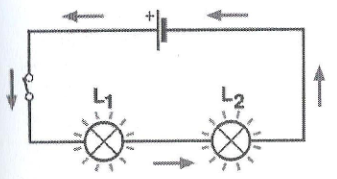
\includegraphics[width=\linewidth]{circuito-serie}
\end{minipage}% Don't leave empty lines and empty chars between minipages
\hfill%
\begin{minipage}[t]{0.45\textwidth}\vspace{0pt}
Montaje en serie significa que el
de tal manera que la misma corriente
la misma corriente pase a través de ellos
 uno tras otro.
La corriente es la misma en todo el
circuito, mientras que la tensión en
terminales de la batería es igual a la suma
de las tensiones en los bornes de cada
lámpara.
\end{minipage}

\item En paralelo (o en derivación)

\noindent\begin{minipage}[t]{0.5\textwidth}\vspace{0pt}
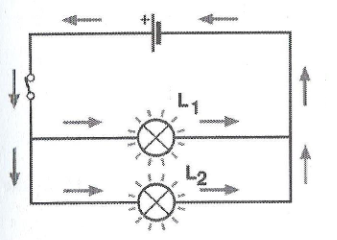
\includegraphics[width=\linewidth]{circuito-paralelo}
\end{minipage}% Don't leave empty lines and empty chars between minipages
\hfill%
\begin{minipage}[t]{0.45\textwidth}\vspace{0pt}
La conexión en paralelo significa que
los dos polos de cada elemento están conectados entre sí.
La corriente suministrada por la batería se
dividida en dos partes para cada una de las lámparas.
Sin embargo, la tensión en los bornes de cada lámpara es la misma que la de la batería.
\end{minipage}
\end{itemize}
Es importante entender la diferencia entre estas dos asociaciones de elementos (o componentes electrónicos) porque no se comprobarán estos elementos de la misma manera en ambos casos.
Por ejemplo, en conexión en paralelo, si mide un cortocircuito en los terminales de L1, quizás sea L2 y no L1 el que tenga la culpa. Deberá desconectar una de estas lámparas para comprobarlo.
\newpage
